\documentclass[10pt,twocolumn,letterpaper]{article}

\usepackage{cvpr}
\usepackage{times}
\usepackage{epsfig}
\usepackage{graphicx}
\usepackage{amsmath}
\usepackage{amssymb}
\usepackage{newfloat}
\usepackage{float}
\graphicspath{{images/}}
\DeclareFloatingEnvironment[%
	fileext=los,
	name=Exhibit,
]{exhibit}

% Include other packages here, before hyperref.

% If you comment hyperref and then uncomment it, you should delete
% egpaper.aux before re-running latex.  (Or just hit 'q' on the first latex
% run, let it finish, and you should be clear).
\usepackage[breaklinks=true,bookmarks=false]{hyperref}

\cvprfinalcopy % *** Uncomment this line for the final submission

\def\cvprPaperID{****} % *** Enter the CVPR Paper ID here
\def\httilde{\mbox{\tt\raisebox{-.5ex}{\symbol{126}}}}

% Pages are numbered in submission mode, and unnumbered in camera-ready
%\ifcvprfinal\pagestyle{empty}\fi
\setcounter{page}{4321}
\begin{document}

%%%%%%%%% TITLE
\title{Recommendation Systems for Movies with Sentiment Analysis using Neural Networks}

\author{Colby Wise\\
Columbia University\\
{\tt\small cjw2165@columbia.edu}
% For a paper whose authors are all at the same institution,
% omit the following lines up until the closing ``}''.
% Additional authors and addresses can be added with ``\and'',
% just like the second author.
% To save space, use either the email address or home page, not both
\and
Michael Alvarino\\
Columbia University\\
{\tt\small maa2282@columbia.edu}
\and
Richard Dewey\\
Columbia University\\
{\tt\small rld2126@columbia.edu}
}

\maketitle
%\thispagestyle{empty}

%%%%%%%%% ABSTRACT
\begin{abstract}
   In this research paper we apply the methodology outlined in the
   arXiv working paper: "Joint Deep Modeling of Users and Items Using Reviews for Recommendation" 
   for rating prediction of movies. The approach used in this paper
   models users and items jointly using review text in two cooperative neural networks.  
   We have extended their model by implementing a different architecture and 
   objective function. We plan to further extend it by testing different hyperparameters
   and architectures.
\end{abstract}

%%%%%%%%% BODY TEXT
\section{Introduction}

Our initial milestone recreated the 
DeepCoNN model outline in the JDM paper using texts reviews for movies from 
the Amazon Instant Video dataset. The results of this recreated model 
will serve as a baseline for model comparison and evaluation.
For the milestone we made a number of small improvements to the model
   
   Source Code:: \href{https://github.com/michaelAlvarino/Deep-Learning}
   {Joint Deep Modeling of Users and Items Using Reviews}

%-------------------------------------------------------------------------

\subsection{Related Work}
\par The literature on recommendation systems is deep and until recently has traditionally focused on well-known matrix factorization algorithms, such as collaborative filtering, as popularized by Netflix and Spotify \href{https://arxiv.org/pdf/1205.3193.pdf}{[Lee, et. al., 2012]}. The benefits of collaborative filtering is that it is relatively easy to implement and computationally efficient given most similarity measure i.e. cosine similarity is matrix multiplication. Conversely, the draw backs in real-world applications have significant implications: namely CF suffers from the "cold-start" problem in that it requires user ratings to make predictions. For instance, for new users without prior history it's hard to predict ratings/recommendations thus models have poor generalization \href{https://cs224d.stanford.edu/reports/BalakrishnanDixit.pdf}{[Balakrishnan, Dixit, 2016]} 

\par Recent research has focused on using Deep Learning, specifically convolutional and recurrent neural networks to help solve the generalization problem. Specifically, we will be focusing on expanding the Deep Cooperative Neural Networks (Deep-CoNN) model thus our primary reference will be the original \href{https://arxiv.org/pdf/1701.04783.pdf}{[Zheng, Noroozi, et. al. 2017]} paper. The authors do not provide their code online, but other have recreated it for video games reviews here \href{https://www.tensorflow.org/tutorials/wide_and_deep}{Joint and Deep}. Additional related papers that we referenced for constructing the Deep portion of our network include DeepFM \href{https://arxiv.org/pdf/1703.04247.pdf}{[Guo, Tang, et. al. 2017]} which similar to our model, combines a matrix factorization with a CNN architecture; and TransNets \href{https://arxiv.org/pdf/1704.02298.pdf}{[Catherine and Cohen. 2017]}, which extends DeepCoNN to examples where the users review is not available. 

It should be noted that our original proposal was to build and improved model of Google's Wide and Deep model. We spent a considerable amount of time going down this path, but ultimately came to the conclusion that we could not source the high quality categorical data needed for training the wide part of the model. We decided to switch to the DeepConn model due to it's improved performance and the availability of high quality data for training, although the model is more complex and will likely be computationally more expensive to train.

%-------------------------------------------------------------------------
\subsection{Problem Formulation}

\textit{In order to make better movie recommendations how can we more accurately predict a users rating for an unseen movie based on what the user has previously seen? Furthermore, can we improve generalization of our model when information on a users past movie ratings is limited?}

These two questions are the crux of our problem. Prior to deep learning, standard approaches for recommendation systems ($RecSys$) used collaborative filtering which relies on decomposing users, items (i.e. movies), and ratings into latent feature matrices. Then the weights of these matrices are used to predict a rating a user would give for an item. One common method includes using the cosine similarity measure between all pairs of movies that users have rated:

Where,\\
\begin{center}
$m_{i}$ and $m_{j}$ refer to movie1/movie2 and denote vectors of ratings from users have rated both movies:\\
\ \newline
\textbf{sim($m_{i}$,$m_{j}$)} = \textbf{$cos(\theta)$} =
$\frac{\vec{m_{i}} \bullet \vec{m_{j}}}{||\vec{m_{i}}||_2 \times ||\vec{m_{j}}||_2}$

\end{center}

This yields a movie-to-movie similarity matrix of dimensions $M \times M$ with ones along the diagonal. Thus, the predicted rating for movie $m_{2}$for user1 would be calculated using similarity measures between ($m_2,m_1$) and ($m_2,m_3$) weighted by the respective ratings for $m_1$ and $m_3$. 

From the above formulation we can clearly see the major disadvantage of this approach: sparsity. When ratings are limited the movie-to-movie matrix is mainly zeros thus limiting predictive ability. In recent years a researcher have attempted to work around this limitation by using text data that users write after watching movies. This text data is used as input for training neural networks and offers additional insights to simple numerical ratings or categorical features. 

The DeepCoNN model formulation that we'll focus on in this research uses two jointly modeled neural networks. The first network $Net_{i}$ uses all of the text reviews for a given user. The second network $Net_{p}$ uses all of the text reviews for a particular product (movie).


\subsection{Data and Methodology}

By modifying a code base found online \href{https://github.com/Praznat/uifud/tree/291b0882b02bf77edf9b310aeeb345784113b1f5}{Join and Deep} we were able to replicate one of the base-case scenarios for the DeepCoNN model. The original code base was incomplete and not well suited for our data, thus our reconfiguring of the DeepCoNN model presented a number of technical challenges. First, we used GloVe (50) to transform our reviews into a vector representation. GloVe returns a matrix representation for each word, so to get the data into the same form as that which is presented in the paper, we take the mean of each column in the GloVe word matrix. Thus for each review we have N words in the review and 50 columns for an N x 50 matrix.

The second technical issue to work through is combining the two networks into a single loss function. This aspect is key to this model and others designed to combine the results of two (or more) neural networks and train them jointly with a common loss function. A number of approaches exist, but as a first step, we tested the baseline implementation of the model, by taking the dot product of the output from the fully connected layer of $Net_{i}$ and output from the fully connected of $Net_{p}$. This method is straightforward to implement, but suffers from the fact that doesn't capture higher level interactions between features. For our final project we plan to implement more robust methods for jointly modeling two neural networks, including using a factorization machine. The the CNN architecture described in the DeepCoNN paper was built using Keras and many of the Keras native methods. 

\subsection{Architecture}

The first layer of the network items (movies are represented as matrices of word embeddings as discussed above. The next layers are standard to CNN's including the convolution, max pooling and fully connected layers.  We use ReLU activations for each convolutional layer as is standard in the literature. The output of each network is joined by taking the dot product of $X_{u}$ and $Y_{i}$ the output vectors of the two neural networks. The approach explained in the paper introduces a shared layer, which allows us to map the two vectors into the same feature space. This is accomplished by concatenating the two vectors $X_{u}$ and $Y_{i}$ and then estimating a factorization machine on the resulting vector $Z$. As described in the paper, we optimize the model using RMSprop, which is an adaptive version of gradient descent that controls the step size with respect to the absolute value of the gradient. The current implementation does not use regularization, however we plan to implement regularization into our final project. 

\subsection{Preliminary Results}

Our preliminary work toward the milestone consisted of reconstructing aspects of the code as highlighted above to model text review data. We confirmed the results reported in the Joint Deep Modeling paper for the DeepCoNN-DP implementation and extended the original DeepCoNN by using alternative hyperparameters of the original architecture that are detailed in Exhibit 1. 

\subsection{Further Research}

For our final project we intended to test various methods for building a shared layer between in the two networks, including a factorization machine. We also intended to test other hyperparameter setting and potentially different architectures including an LSTM structure. Finally, as a robustness check, we intend to test our model on other datasets, including the amazon TV and video games datasets. Both of these datasets have similarly structured text reviews and should be amenable to the DeppCoNN predictive model. 

\section{Diagrams}
\paragraph{Model Diagram} \ \newline
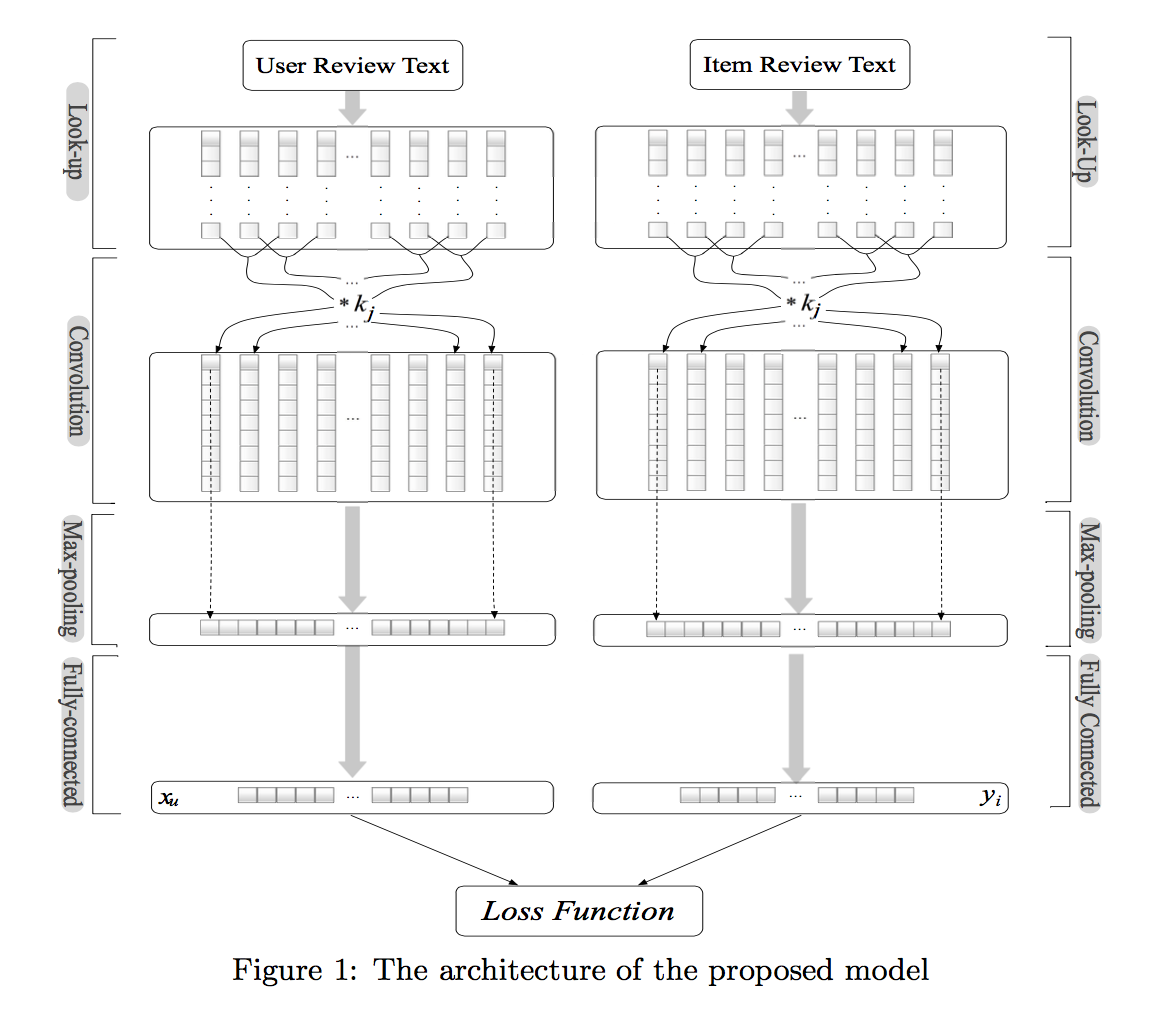
\includegraphics[scale=0.38]{DeepCoNN}


%\FloatBarrier
\begin{exhibit}
\begin{center}
{\small
\begin{tabular}{l|ccccccc}
\hline
%Category & Experiment Summary  \\ \hline
Model & Losses & Training Time & & & &  &\\
\hline
DeepCoNN-DP\footnote{DP is the dot product implementation} & & & & & & & \\
Stand Alone FM & & & & & & &\\
\hline
\end{tabular}
}
\end{center}
\label{table2}
\caption{Model Summary}
\end{exhibit}

\subsection{References}

[1] Zheng, Lei, Noroozi, Vahid and Yu, Philip. Joint Deep Modeling of Users
 and Items Using Reviews for Recommendations. arXiv working paper. June 2017

[2] Rendle, Steffan. Factorization Machines. ICDM 2010

[3] Catherine, Rose and Cohen, William. TransNets: Learning to Transform
for Recommendation. arXiv working paper. June 2017

[4] D. Agarwal and B.-C. Chen. Regression-based latent
factor models. In KDD, pages 19?28, 2009.

[5] P. Baldi and P. J. Sadowski. Understanding dropout.
In NIPS, pages 2814?2822, 2013.

[6] Y. Bengio, L. Yao, G. Alain, and P. Vincent.
Generalized denoising auto-encoders as generative
models. In NIPS, pages 899?907, 2013.

[7] C. M. Bishop. Pattern Recognition and Machine
Learning. Springer-Verlag New York, Inc., Secaucus,
NJ, USA, 2006.


\end{document}



AIV\footnote{Amazon Instant Video}
DeepCoNN-DP X-layer & AIV & & & & & &\\
DeepCoNN & AIV & & & & & &\\
DeepCoNN X layer & AIV & & & & & &\\
DeepCoNN & TV & & & & & &\\
DeepCoNN & Video Games & & & & & &\\

Please number all of your sections and displayed equations.  It is
important for readers to be able to refer to any particular equation.  Just
because you didn't refer to it in the text doesn't mean some future reader
might not need to refer to it.  It is cumbersome to have to use
circumlocutions like ``the equation second from the top of page 3 column
1''.  (Note that the ruler will not be present in the final copy, so is not
an alternative to equation numbers).  All authors will benefit from reading
Mermin's description of how to write mathematics:
\url{http://www.pamitc.org/documents/mermin.pdf}.


\subsection{Preliminary Results}
\begin{figure}[t]
\begin{center}
%\fbox{\rule{0pt}{2in} \rule{0.9\linewidth}{0pt}
 \fbox{  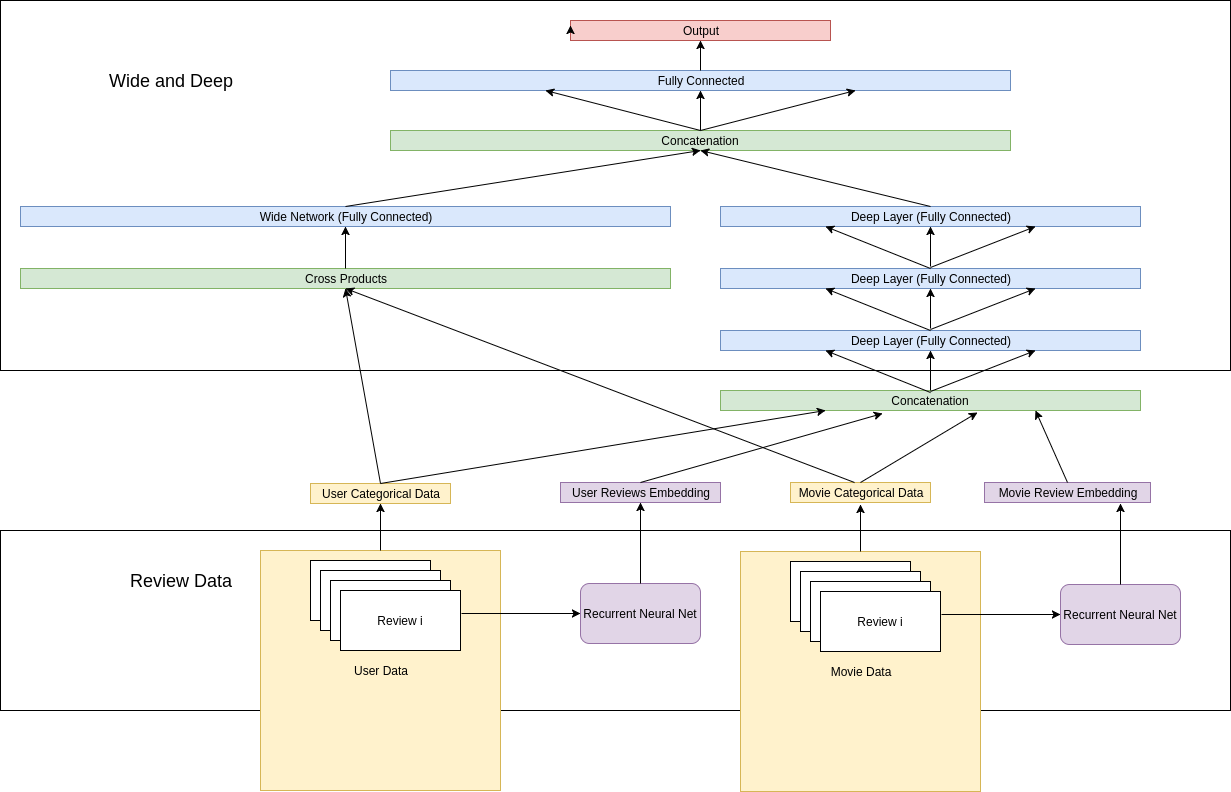
\includegraphics[width=1.0\linewidth]{network_diagram}}
\end{center}
   \caption{Example of caption.  It is set in Roman so that mathematics
   (always set in Roman: $B \sin A = A \sin B$) may be included without an
   ugly clash.}
\label{fig:long}
\label{fig:onecol}
\end{figure}
Many authors misunderstand the concept of anonymizing for blind
review.  Blind review does not mean that one must remove
citations to one's own work---in fact it is often impossible to
review a paper unless the previous citations are known and
available.

Blind review means that you do not use the words ``my'' or ``our''
when citing previous work.  That is all.  (But see below for
techreports.)

Saying ``this builds on the work of Lucy Smith [1]'' does not say
that you are Lucy Smith; it says that you are building on her
work.  If you are Smith and Jones, do not say ``as we show in
[7]'', say ``as Smith and Jones show in [7]'' and at the end of the
paper, include reference 7 as you would any other cited work.

An example of a bad paper just asking to be rejected:
\begin{quote}
\begin{center}
    An analysis of the frobnicatable foo filter.
\end{center}

   In this paper we present a performance analysis of our
   previous paper [1], and show it to be inferior to all
   previously known methods.  Why the previous paper was
   accepted without this analysis is beyond me.

   [1] Removed for blind review
\end{quote}


An example of an acceptable paper:

\begin{quote}
\begin{center}
     An analysis of the frobnicatable foo filter.
\end{center}

   In this paper we present a performance analysis of the
   paper of Smith \etal [1], and show it to be inferior to
   all previously known methods.  Why the previous paper
   was accepted without this analysis is beyond me.

   [1] Smith, L and Jones, C. ``The frobnicatable foo
   filter, a fundamental contribution to human knowledge''.
   Nature 381(12), 1-213.
\end{quote}

If you are making a submission to another conference at the same time,
which covers similar or overlapping material, you may need to refer to that
submission in order to explain the differences, just as you would if you
had previously published related work.  In such cases, include the
anonymized parallel submission~\cite{Authors14} as additional material and
cite it as
\begin{quote}
[1] Authors. ``The frobnicatable foo filter'', F\&G 2014 Submission ID 324,
Supplied as additional material {\tt fg324.pdf}.
\end{quote}

Finally, you may feel you need to tell the reader that more details can be
found elsewhere, and refer them to a technical report.  For conference
submissions, the paper must stand on its own, and not {\em require} the
reviewer to go to a techreport for further details.  Thus, you may say in
the body of the paper ``further details may be found
in~\cite{Authors14b}''.  Then submit the techreport as additional material.
Again, you may not assume the reviewers will read this material.

Sometimes your paper is about a problem which you tested using a tool which
is widely known to be restricted to a single institution.  For example,
let's say it's 1969, you have solved a key problem on the Apollo lander,
and you believe that the CVPR70 audience would like to hear about your
solution.  The work is a development of your celebrated 1968 paper entitled
``Zero-g frobnication: How being the only people in the world with access to
the Apollo lander source code makes us a wow at parties'', by Zeus \etal.

You can handle this paper like any other.  Don't write ``We show how to
improve our previous work [Anonymous, 1968].  This time we tested the
algorithm on a lunar lander [name of lander removed for blind review]''.
That would be silly, and would immediately identify the authors. Instead
write the following:
\begin{quotation}
\noindent
   We describe a system for zero-g frobnication.  This
   system is new because it handles the following cases:
   A, B.  Previous systems [Zeus et al. 1968] didn't
   handle case B properly.  Ours handles it by including
   a foo term in the bar integral.

   ...

   The proposed system was integrated with the Apollo
   lunar lander, and went all the way to the moon, don't
   you know.  It displayed the following behaviours
   which show how well we solved cases A and B: ...
\end{quotation}
As you can see, the above text follows standard scientific convention,
reads better than the first version, and does not explicitly name you as
the authors.  A reviewer might think it likely that the new paper was
written by Zeus \etal, but cannot make any decision based on that guess.
He or she would have to be sure that no other authors could have been
contracted to solve problem B.
\medskip

\noindent
FAQ\medskip\\
{\bf Q:} Are acknowledgements OK?\\
{\bf A:} No.  Leave them for the final copy.\medskip\\
{\bf Q:} How do I cite my results reported in open challenges?
{\bf A:} To conform with the double blind review policy, you can report results of other challenge participants together with your results in your paper. For your results, however, you should not identify yourself and should not mention your participation in the challenge. Instead present your results referring to the method proposed in your paper and draw conclusions based on the experimental comparison to other results.\medskip\\



\begin{figure}[t]
\begin{center}
 \fbox{  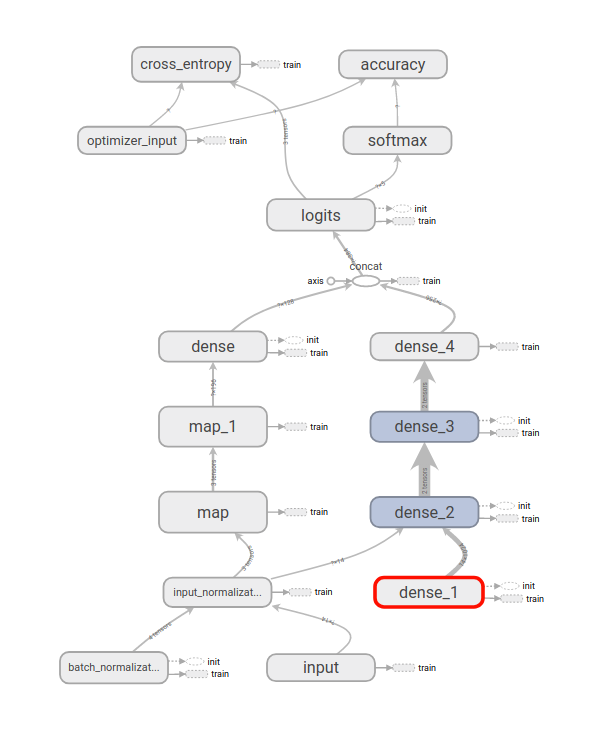
\includegraphics[width=1.0\linewidth]{TFBoardNetwork}}
\end{center}
   \caption{Example of caption.  It is set in Roman so that mathematics
   (always set in Roman: $B \sin A = A \sin B$) may be included without an
   ugly clash.}
\label{fig:long}
\label{fig:onecol}
\end{figure}

\subsection{Miscellaneous}

\noindent
Compare the following:\\
\begin{tabular}{ll}
 \verb'$conf_a$' &  $conf_a$ \\
 \verb'$\mathit{conf}_a$' & $\mathit{conf}_a$
\end{tabular}\\
See The \TeX book, p165.

The space after \eg, meaning ``for example'', should not be a
sentence-ending space. So \eg is correct, {\em e.g.} is not.  The provided
\verb'\eg' macro takes care of this.

When citing a multi-author paper, you may save space by using ``et alia'',
shortened to ``\etal'' (not ``{\em et.\ al.}'' as ``{\em et}'' is a complete word.)
However, use it only when there are three or more authors.  Thus, the
following is correct: ``
   Frobnication has been trendy lately.
   It was introduced by Alpher~\cite{Alpher02}, and subsequently developed by
   Alpher and Fotheringham-Smythe~\cite{Alpher03}, and Alpher \etal~\cite{Alpher04}.''

This is incorrect: ``... subsequently developed by Alpher \etal~\cite{Alpher03} ...''
because reference~\cite{Alpher03} has just two authors.  If you use the
\verb'\etal' macro provided, then you need not worry about double periods
when used at the end of a sentence as in Alpher \etal.

For this citation style, keep multiple citations in numerical (not
chronological) order, so prefer \cite{Alpher03,Alpher02,Authors14} to
\cite{Alpher02,Alpher03,Authors14}.


\begin{figure*}
\begin{center}
\fbox{\rule{0pt}{2in} \rule{.9\linewidth}{0pt}}
\end{center}
   \caption{Example of a short caption, which should be centered.}
\label{fig:short}
\end{figure*}

%------------------------------------------------------------------------
\section{Formatting your paper}

All text must be in a two-column format. The total allowable width of the
text area is $6\frac78$ inches (17.5 cm) wide by $8\frac78$ inches (22.54
cm) high. Columns are to be $3\frac14$ inches (8.25 cm) wide, with a
$\frac{5}{16}$ inch (0.8 cm) space between them. The main title (on the
first page) should begin 1.0 inch (2.54 cm) from the top edge of the
page. The second and following pages should begin 1.0 inch (2.54 cm) from
the top edge. On all pages, the bottom margin should be 1-1/8 inches (2.86
cm) from the bottom edge of the page for $8.5 \times 11$-inch paper; for A4
paper, approximately 1-5/8 inches (4.13 cm) from the bottom edge of the
page.

%-------------------------------------------------------------------------
\subsection{Margins and page numbering}

All printed material, including text, illustrations, and charts, must be kept
within a print area 6-7/8 inches (17.5 cm) wide by 8-7/8 inches (22.54 cm)
high.
Page numbers should be in footer with page numbers, centered and .75
inches from the bottom of the page and make it start at the correct page
number rather than the 4321 in the example.  To do this fine the line (around
line 23)
\begin{verbatim}
%\ifcvprfinal\pagestyle{empty}\fi
\setcounter{page}{4321}
\end{verbatim}
where the number 4321 is your assigned starting page.

Make sure the first page is numbered by commenting out the first page being
empty on line 46
\begin{verbatim}
%\thispagestyle{empty}
\end{verbatim}


%-------------------------------------------------------------------------
\subsection{Type-style and fonts}

Wherever Times is specified, Times Roman may also be used. If neither is
available on your word processor, please use the font closest in
appearance to Times to which you have access.

MAIN TITLE. Center the title 1-3/8 inches (3.49 cm) from the top edge of
the first page. The title should be in Times 14-point, boldface type.
Capitalize the first letter of nouns, pronouns, verbs, adjectives, and
adverbs; do not capitalize articles, coordinate conjunctions, or
prepositions (unless the title begins with such a word). Leave two blank
lines after the title.

AUTHOR NAME(s) and AFFILIATION(s) are to be centered beneath the title
and printed in Times 12-point, non-boldface type. This information is to
be followed by two blank lines.

The ABSTRACT and MAIN TEXT are to be in a two-column format.

MAIN TEXT. Type main text in 10-point Times, single-spaced. Do NOT use
double-spacing. All paragraphs should be indented 1 pica (approx. 1/6
inch or 0.422 cm). Make sure your text is fully justified---that is,
flush left and flush right. Please do not place any additional blank
lines between paragraphs.

Figure and table captions should be 9-point Roman type as in
Figures~\ref{fig:onecol} and~\ref{fig:short}.  Short captions should be centred.

\noindent Callouts should be 9-point Helvetica, non-boldface type.
Initially capitalize only the first word of section titles and first-,
second-, and third-order headings.

FIRST-ORDER HEADINGS. (For example, {\large \bf 1. Introduction})
should be Times 12-point boldface, initially capitalized, flush left,
with one blank line before, and one blank line after.

SECOND-ORDER HEADINGS. (For example, { \bf 1.1. Database elements})
should be Times 11-point boldface, initially capitalized, flush left,
with one blank line before, and one after. If you require a third-order
heading (we discourage it), use 10-point Times, boldface, initially
capitalized, flush left, preceded by one blank line, followed by a period
and your text on the same line.

%-------------------------------------------------------------------------
\subsection{Footnotes}

Please use footnotes\footnote {This is what a footnote looks like.  It
often distracts the reader from the main flow of the argument.} sparingly.
Indeed, try to avoid footnotes altogether and include necessary peripheral
observations in
the text (within parentheses, if you prefer, as in this sentence).  If you
wish to use a footnote, place it at the bottom of the column on the page on
which it is referenced. Use Times 8-point type, single-spaced.


%-------------------------------------------------------------------------
\subsection{References}

List and number all bibliographical references in 9-point Times,
single-spaced, at the end of your paper. When referenced in the text,
enclose the citation number in square brackets, for
example~\cite{Authors14}.  Where appropriate, include the name(s) of
editors of referenced books.

\begin{table}
\begin{center}
\begin{tabular}{|l|c|}
\hline
Method & Frobnability \\
\hline\hline
Theirs & Frumpy \\
Yours & Frobbly \\
Ours & Makes one's heart Frob\\
\hline
\end{tabular}
\end{center}
\caption{Results.   Ours is better.}
\end{table}

%-------------------------------------------------------------------------
\subsection{Illustrations, graphs, and photographs}

All graphics should be centered.  Please ensure that any point you wish to
make is resolvable in a printed copy of the paper.  Resize fonts in figures
to match the font in the body text, and choose line widths which render
effectively in print.  Many readers (and reviewers), even of an electronic
copy, will choose to print your paper in order to read it.  You cannot
insist that they do otherwise, and therefore must not assume that they can
zoom in to see tiny details on a graphic.

When placing figures in \LaTeX, it's almost always best to use
\verb+\includegraphics+, and to specify the  figure width as a multiple of
the line width as in the example below
{\small\begin{verbatim}
   \usepackage[dvips]{graphicx} ...
   \includegraphics[width=0.8\linewidth]
                   {myfile.eps}
\end{verbatim}
}


%-------------------------------------------------------------------------
\subsection{Color}

Please refer to the author guidelines on the CVPR 2018 web page for a discussion
of the use of color in your document.

%------------------------------------------------------------------------
\section{Final copy}

You must include your signed IEEE copyright release form when you submit
your finished paper. We MUST have this form before your paper can be
published in the proceedings.

Please direct any questions to the production editor in charge of these
proceedings at the IEEE Computer Society Press: Phone (714) 821-8380, or
Fax (714) 761-1784.

{\small
\bibliographystyle{ieee}
\bibliography{egbib}
}

\end{document}
